\section{Quantitaive Evaluation}
\label{sec:oc_quant}

\subsection{Image classification}

\paragraph{CNN}
\autoref{tab:imagenet-cnn} shows ImageNet classification metrics using \Th{VGG16} and \Th{ResNet50}.
 Our Opti-CAM brings impressive performance in terms of \glsfirst{ad} and Average Increase 
 \gls{ai} metrics. That is, not only impressive improvement over baselines, but near-perfect: 
 near-zero $\AD$ and above 90\% $\AI$. Our new metric $\AG$ is lower, around 70\% 
 for Opti-CAM, but this is still several times higher than for all the other methods.\\
%--------------------------------------------------------------------------------------------------
%------------------------------------------------------------------------------
\begin{table}
\centering
\footnotesize
\setlength{\tabcolsep}{4pt}
\renewcommand{\arraystretch}{0.8}
\begin{tabular}{lrrrr|rrrr} \toprule
\mr{2}{\Th{Method}}                                & \mc{4}{\Th{ResNet50}} & \mc{4}{\Th{VGG16}} \\ \cmidrule{2-9}
                                                   & {$\AD\!\downarrow$} & {$\AG\!\uparrow$} & {$\AI\!\uparrow$} & \mc{1}{T} & {$\AD\!\downarrow$} & {$\AG\!\uparrow$} & {$\AI\!\uparrow$} & \mc{1}{T} \\ \midrule
Fake-CAM                &  0.8 &  1.6 & 46.0 &  0.00 &  0.5 &  0.6 & 42.6 &  0.00 \\ \midrule
Grad-CAM                & 12.2 & 17.6 & 44.4 &  0.03 & 14.2 & 14.7 & 40.6 &  0.02 \\
Grad-CAM++              & 12.9 & 16.0 & 42.1 &  0.03 & 17.1 & 10.2 & 33.4 &  0.02 \\
Score-CAM               &  8.6 & 26.6 & 56.7 & 15.22 & 13.5 & 15.6 & 41.7 &  3.11 \\
Ablation-CAM            & 12.5 & 16.4 & 42.8 & 18.26 & 15.5 & 12.6 & 36.9 &  2.98 \\
XGrad-CAM               & 12.2 & 17.6 & 44.4 &  0.03 & 13.8 & 14.8 & 41.2 &  0.02 \\
Layer-CAM               & 15.6 & 15.0 & 38.8 &  0.08 & 48.9 &  3.1 & 13.5 &  0.07 \\
ExPerturbation          & 38.1 &  9.5 & 22.5 & 152.96 & 43.0 &  7.1 & 20.5 & 83.20 \\
\hline
Opti-CAM                & \tb{ 1.5} & \tb{68.8} & \tb{92.8} &  4.15 &  \tb{1.3} & \tb{71.2} & \tb{92.7} & 3.94 \\
\bottomrule
\end{tabular}
\caption{\emph{Classification metrics} on ImageNet validation set, using CNNs. $\AD$/$\AI$: 
average drop/increase \autocite{chattopadhay2018grad}; $\AG$: average gain (ours); 
$\downarrow$ / $\uparrow$: lower / higher is better; 
T: \iavr{Average time (sec) per batch of 8 images. Bold: best, excluding Fake-CAM.}}
\label{tab:imagenet-cnn}
% \vspace{-0.2cm}
\end{table}
%------------------------------------------------------------------------------
% FakeCAM~\citep{poppi2021revisiting}
% Grad-CAM ~\citep{selvaraju2017grad}
% Grad-CAM++~\cite{chattopadhay2018grad}
% ScoreCAM~\citep{wang2020score} 
% AblationCAM~\citep{ramaswamy2020ablation}
% XGrad-CAM~\citep{fu2020axiom} 
% LayerCAM~\citep{jiang2021layercam} 
% ExPerturbation~\citep{fong2019understanding}
%\modify{HiRes-CAM} &\modify{12.2}&\modify{17.6}&\modify{44.4}&\modify{0.03}&\modify{15.8}&\modify{13.2}&\modify{37.8}&\modify{0.02}\\

%--------------------------------------------------------------------------------------------------
\noindent Interestingly, Fake-CAM \autocite{poppi2021revisiting} is the winner in terms of $\AD$ 
and second or third best in $\AI$ after Opti-CAM and Score-CAM, but fails completely $\AG$. This is 
expected and makes Fake-CAM uninteresting as it should be: By only masking one pixel, the 
classification score can hardly drop (0.8\% on ResNet50) and while it increases very often (on 
46\% of images), the gain is as little as the drop (0.7\%). This makes the pair ($\AD$, $\AG$) 
sufficient as primary metrics and $\AI$ can be thought of as secondary, if important at all.\\

%In the supplementary material we report \emph{insertion} (I) and \emph{deletion} (D) metrics along with failure cases of Opti-CAM. The latter indicate that our saliency maps are not incorrect as a whole, but capturing more parts of the object, more instances or more background context results in larger or several disconnected salient regions. This does not let the classifier focus on a single discriminative region when pixels are processed sequentially by increasing saliency. Rather, I/D favor smaller and more compact saliency maps.


\noindent \autoref{tab:imagenet-cnn} also includes average execution time per image over the 1000-image 
ImageNet subset for all methods. Opti-CAM is slower than gradient-based methods that require 
only one pass through the network, but on par or faster than gradient-free methods. 
Indeed, we use a maximum of 100 iterations with one forward/backward pass per iteration, 
while Score-CAM and Ablation-CAM perform as many forward passes as channels. Hence, they are much 
slower on ResNet50 than VGG16. Extremal Perturbation does not depend on the number of channels but 
is very slow by performing a complex optimization in the image space.

\paragraph{Transformers}
\autoref{tab:imagenet-trans} shows ImageNet classification metrics using ViT \iavr{and DeiT}. 
Unlike CAM-based methods that rely on a class-specific linear combination of feature maps, 
raw attention \autocite{dosovitskiy2020image} and rollout \autocite{abnar2020quantifying} use the 
attention map of the [CLS] token from the last attention block and from all blocks respectively. 
This attention map depends only on the particular image and not on the target class, hence it 
is not really comparable. TIBAV \autocite{chefer2021transformer} uses both instance-specific and 
class-specific information.
%--------------------------------------------------------------------------------------------------
%------------------------------------------------------------------------------
\begin{table}
    \centering
    \footnotesize
    \setlength{\tabcolsep}{4pt}
    \renewcommand{\arraystretch}{0.8}
    \begin{tabular}{lrrrr|rrrr} \toprule
        \mr{2}{\Th{Method}}& \mc{4}{\Th{ViT-B}} & \mc{4}{\Th{DeiT-B}} \\ \cmidrule{2-9}
        & {$\AD\!\downarrow$} & {$\AG\!\uparrow$} & {$\AI\!\uparrow$} & \mc{1}{T} & {$\AD\!\downarrow$} & {$\AG\!\uparrow$} & {$\AI\!\uparrow$} & \mc{1}{T} \\ \midrule
        Fake-CAM            &  0.3 &  0.4 & 48.3 &  0.00 &  0.6 &  0.3 & 44.6 &  0.00 \\ \midrule
        Grad-CAM            & 69.4 &  2.5 & 12.4 &  0.14 & 33.5 &  1.7 & 12.5 &  0.11 \\
        Grad-CAM            & 86.3 &  1.5 &  1.0 &  0.15 & 50.7 &  0.9 &  7.2 &  0.13 \\
        Score-CAM           & 32.0 &  6.2 & 33.0 & 23.69 & 53.6 &  2.2 & 12.2 & 22.47 \\
        XGrad-CAM           & 88.1 &  0.4 &  4.3 &  0.13 & 80.5 &  0.3 &  4.1 &  0.12 \\
        Layer-CAM           & 82.0 &  0.2 &  2.9 &  0.24 & 88.9 &  0.4 &  2.6 & 0.24\\
        ExPerturbation      &28.8&6.2&24.4&133.52&60.9&2.0&8.5&129.12\\
        RawAtt              & 92.6 &  0.2 &  2.8 &  0.02 & 95.3 &  0.0 &  1.8 &  0.02 \\
        Rollout             & 42.1 &  5.6 & 20.9 &  0.02 & 55.2 &  0.8 &  7.9 &  0.02 \\
        TIBAV               & 81.7 &  0.8 &  5.8 &  0.16 & 62.3 &  0.7 &  7.1 &  0.16 \\\midrule
        Opti-CAM            & \tb{ 0.6} &   \tb{18.0} & \tb{90.1} &    16.05 & \tb{ 0.9} & \tb{26.0} & \tb{83.5} &    15.17 \\ \bottomrule
    \end{tabular}
    \caption{}
    %\caption{\emph{Classification metrics} on ImageNet validation set, using transformers. $\AD$/$\AI$: average drop/increase
    %\autocite{chattopadhay2018grad}; $\AG$: average gain (ours); $\downarrow$ / $\uparrow$: lower / higher is better. \iavr{T: Average time (sec) per batch of 8 images. Bold: best, excluding Fake-CAM.}}
    \label{tab:imagenet-trans}
\end{table}
%------------------------------------------------------------------------------
%Fake-CAM~\citep{poppi2021revisiting}    &  0.3 &  0.4 & 48.3 &  0.00 &  0.6 &  0.3 & 44.6 &  0.00 \\ \midrule
%Grad-CAM~\citep{selvaraju2017grad}      & 69.4 &  2.5 & 12.4 &  0.14 & 33.5 &  1.7 & 12.5 &  0.11 \\
%Grad-CAM++~\cite{chattopadhay2018grad}  & 86.3 &  1.5 &  1.0 &  0.15 & 50.7 &  0.9 &  7.2 &  0.13 \\
%Score-CAM~\citep{wang2020score}         & 32.0 &  6.2 & 33.0 & 23.69 & 53.6 &  2.2 & 12.2 & 22.47 \\
%XGrad-CAM~\citep{fu2020axiom}           & 88.1 &  0.4 &  4.3 &  0.13 & 80.5 &  0.3 &  4.1 &  0.12 \\
%Layer-CAM~\citep{jiang2021layercam}     & 82.0 &  0.2 &  2.9 &  0.24 & 88.9 &  0.4 &  2.6 & 0.24\\
%ExPerturbation~\citep{fong2019understanding}&28.8&6.2&24.4&133.52&60.9&2.0&8.5&129.12\\
%RawAtt~\citep{dosovitskiy2020image}     & 92.6 &  0.2 &  2.8 &  0.02 & 95.3 &  0.0 &  1.8 &  0.02 \\
%Rollout~\citep{abnar2020quantifying}    & 42.1 &  5.6 & 20.9 &  0.02 & 55.2 &  0.8 &  7.9 &  0.02 \\
%TIBAV~\cite{chefer2021transformer}      & 81.7 &  0.8 &  5.8 &  0.16 & 62.3 &  0.7 &  7.1 &  0.16 \\
%\modify{HiRes-CAM~\citep{draelos2020use}} &\modify{98.4}&\modify{0.0}&\modify{0.7}&\modify{0.03}&\modify{97.2}&\modify{0.0}&\modify{1.2}&\modify{0.03} \\
%\hline
%Opti-CAM (ours)                         & \tb{ 0.6} &   \tb{18.0} & \tb{90.1} &    16.05 & \tb{ 0.9} & \tb{26.0} & \tb{83.5} &    15.17 \\ \bottomrule
%--------------------------------------------------------------------------------------------------
Opti-CAM outperforms all other methods dramatically, reaching near-zero $\AD$ and $\AI$ above 80 or 
90\%. According to our new $\AG$ metric, Opti-CAM still works while all other methods fail, 
but $\AG$ is much more conservative than $\AI$. On ViT-B for example, the classification score 
increases for 90.1\% of the images by masking with Opti-CAM, but the gain is only 18.0\% on average.

\paragraph{More metrics}
In this section, we show additional metrics including AOPC \autocite{samek2016evaluating}, 
Max-Sensitivity\autocite{yeh2019fidelity} and ADCC \autocite{poppi2021revisiting}.

We use the code and suggested parameters of package 
Quantus\footnote{\url{https://github.com/understandable-machine-intelligence-lab/Quantus}} to 
measure AOPC and MS. In particular, patch size $14$ and number of evaluation regions $10$ for AOPC; 
lower bound $0.2$ and number of samples $10$ for MS.
For ADCC, we use the official code\footnote{\url{https://github.com/aimagelab/ADCC}}.\\

\noindent We evaluate these metrics on ImageNet validation set using ResNet50 and VGG16. The results are 
reported in \autoref{tab:more-metrics-asked}. Since AOPC shares the same philosophy as I/D, it is 
not a surprise that Opti-CAM has poor performance on AOPC. Opti-CAM achieves the best performance on MS.
%--------------------------------------------------------------------------------------------------
\begin{table}[t]
    \centering
    \scriptsize
    \setlength{\tabcolsep}{4pt}
    \begin{tabular}{lrrr rrr} \toprule
        \mr{2}{\Th{Method}} & \mc{3}{\Th{ResNet50}} & \mc{3}{\Th{VGG16}}  \\ \cmidrule{2-7}
        & {{$AOPC\uparrow$}} & {{$MS\downarrow$}}& {{$ADCC\downarrow$}} & {{$AOPC\uparrow$}} 
        & {{$MS\downarrow$}}& {{$ADCC\downarrow$}}  \\ \midrule
        Grad-CAM            &11.7&1.05&74.3&13.1&1.10&73.7        \\
        Grad-CAM++          &11.6&1.04&73.6&11.6&1.09&74.6          \\
        Score-CAM           &10.2&1.04&61.0&11.0&1.09&73.9             \\
        XGrad-CAM           &11.9&1.05&74.3&13.1&1.10&73.9           \\
        Ablation-CAM        &11.1&1.04&71.5&12.5&1.10&75.5          \\
        Layer-CAM           &\tb{13.0}&1.22&61.1&\tb{13.3}&1.25&51.7 \\
        ExPerturbation      &12.0&1.07&\tb{26.0}&11.2&1.09&\tb{42.8}  \\\hline
        Opti-CAM (ours)     &6.3&\tb{1.03}&65.5&8.9&\tb{1.06}&70.0        \\ \bottomrule
    \end{tabular}
    %\caption{}
    \caption{\textbf{AOPC/MS/ADCC} scores on ImageNet validation set.}
    \label{tab:more-metrics-asked}
\end{table}
% -------------------------------------------------------------------------------------------------
The experimental results are shown in \autoref{tab:imagenet_cnn_hihd} for CNNs and transformers. 
ExPerturbation \autocite{fong2019understanding} is expected to perform best in insertion because its 
optimization objective is very similar to this evaluation metric, using blurring for masked regions. 
However, ExPerturbation \autocite{fong2019understanding}  only performs best on ResNet50. 
TIBAV \autocite{chefer2021transformer}, which is designed for transformers, outperforms the other 
methods on DeiT and ViT. According to the results of Insertion/Deletion, Opti-CAM has low 
performance, but there is no clear winner on either CNNs or transformers.
% -------------------------------------------------------------------------------------------------
\begin{table}[H]
    \centering
    \scriptsize
    \setlength{\tabcolsep}{8pt}
    \renewcommand{\arraystretch}{0.8}
    \begin{tabular}{lrr rr rr rr} \toprule
    \mr{2}{\Th{Method}} & \mc{2}{\Th{ResNet50}} & \mc{2}{\Th{VGG16}} & \mc{2}{\Th{ViT-B}}& \mc{2}{\Th{DeiT-B}} \\ \cmidrule{2-9}
                        & {{$\I\!\uparrow$}} & {{$\D\!\downarrow$}}& {{$\I\!\uparrow$}} & {{$\D\!\downarrow$}} & {{$\I\!\uparrow$}} & {{$\D\!\downarrow$}}& {{$\I\!\uparrow$}} & {{$\D\!\downarrow$}}\\ \midrule
    Fake-CAM&50.7&28.1&46.1&26.9&57.4&33.3&57.5&34.2\\\midrule
    Grad-CAM&66.3&14.7&\tb{64.1}&11.6&62.9&19.8&61.8&17.5\\
    Grad-CAM++&66.0&14.7&62.9&12.2&56.7&29.3&60.5&21.9\\
    Score-CAM&65.7&16.3&62.5&12.1&\tb{66.5}&15.1 &60.6&24.4\\
    XGrad-CAM&66.3&14.7&\tb{64.1}&11.7&55.6&26.5  &55.2&31.1\\
    %\midrule
    Layer-CAM&67.0&\tb{14.2}&58.3&\tb{6.4}&62.9&14.6 &61.6&21.2\\
    ExPerturbation&\tb{70.7}&15.0&61.1&15.0&64.4&18.4&62.1&27.0\\
    Ablation-CAM&65.9&14.6&63.8&11.4&-&-&-&-\\
    RawAtt&-&-&-&-&62.2&17.9 &56.3&29.3\\
    Rollout&-&-&-&-&64.8&15.2 &56.7&32.8\\
    TIBAV&-&-&-&-&66.1&\tb{14.1} &\tb{63.7}&\tb{16.3}\\
    Opti-CAM (ours)&62.0&19.7&59.2&11.0 &60.5&22.0  &59.2&22.8\\
    \bottomrule
    \end{tabular}
    % \vspace{6pt}
    \caption{\textbf{I/D: insertion/deletion} \autocite{petsiuk2018rise} scores on ImageNet validation set; 
    $\downarrow$ / $\uparrow$: lower / higher is better.}% Bold: best, excluding Fake-CAM.}
    \label{tab:imagenet_cnn_hihd}
\end{table}
% -------------------------------------------------------------------------------------------------
\noindent Insertion/Deletion include 224 steps of binarization, with a set of 224 pixels being 
inserted/deleted at each step. If these pixels are all inserted over a single small area, the 
effect on the classifier is more immediate than when sparsely inserting pixels over multiple areas. 
The same observation holds for deletion. By contrast, Opti-CAM attempts to find regions that 
contribute to the classification as a whole. There is no guarantee that those regions are effective 
when used in isolation.\\

\noindent To further understand the behavior of Opti-CAM, we investigate in \autoref{fig:hihd} 
examples where Score-CAM succeeds (insertion score greater than $90$ and deletion score less than 
$10$) and Opti-CAM fails (insertion score less than $70$ and deletion score greater than $15$). 
Compared with Score-CAM, the saliency maps obtained by Opti-CAM are more spread out and highlight 
several parts of the object and background context. In most of the cases, Opti-CAM fails I/D because 
it not only finds the object but also attaches importance to the background.
% -------------------------------------------------------------------------------------------------
%------------------------------------------------------------------------------
\begin{figure}[H]
    \newcommand{\sizeP}{.12}
    \newcommand{\sizeS}{.12}
    \newcommand{\hh}{.175\textwidth}
    \newcommand{\ww}{.200\textwidth}
    \tiny
    \centering
    \setlength{\tabcolsep}{3pt}
    \begin{tabular}{cccccc}
    \centering
    Original & Opti-CAM & Score-CAM & Original & Opti-CAM & Score-CAM\\
    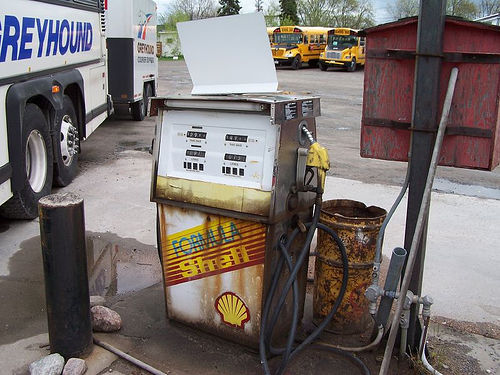
\includegraphics[trim={28mm 8mm 28mm 8mm},clip, width=\sizeP\textwidth]{opticam/images/eval/hihd/ILSVRC2012_val_00045353.JPEG}
    &
    \fig[\sizeS]{opticam/images/eval/hihd/ILSVRC2012_val_00045353JPEG_smap_opticam.png} 
    &  
    \fig[\sizeS]{opticam/images/eval/hihd/ILSVRC2012_val_00045353JPEG_smap_scorecam.png} &
    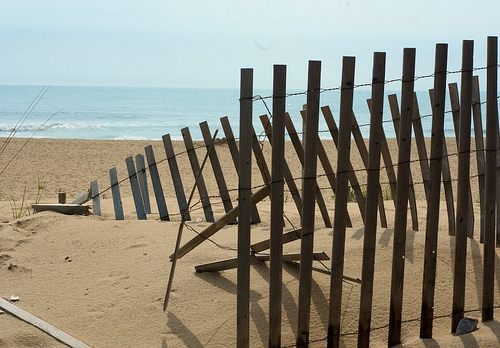
\includegraphics[trim={32mm 14mm 36mm 1mm},clip, width=\sizeP\textwidth]{opticam/images/eval/hihd/ILSVRC2012_val_00041066.JPEG}
    &
    \fig[\sizeS]{opticam/images/eval/hihd/ILSVRC2012_val_00041066JPEG_smap_opticam.png} 
    &          
    \fig[\sizeS]{opticam/images/eval/hihd/ILSVRC2012_val_00041066JPEG_smap_scorecam.png} \\
    gas pump&I$\uparrow$:66.3, D$\downarrow$:19.4&I$\uparrow$:94.2, D$\downarrow$:9.4&
    worm fence&I$\uparrow$:69.7, D$\downarrow$:16.8&I$\uparrow$:91.9, D$\downarrow$:4.4\\
    &AG$\uparrow$:100.0, AD$\downarrow$:0.0&AG$\uparrow$:0.0, AD$\downarrow$:0.0&
    &AG$\uparrow$:73.2, AD$\downarrow$:0.0&AG$\uparrow$:0.0, AD$\downarrow$:28.8\\
    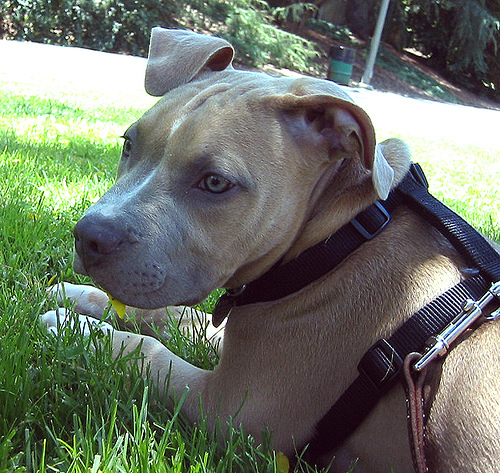
\includegraphics[trim={10mm 14mm 10mm 4mm},clip, width=\sizeP\textwidth]{opticam/images/eval/hihd/ILSVRC2012_val_00040673.JPEG}
    &        
    \fig[\sizeS]{opticam/images/eval/hihd/ILSVRC2012_val_00040673JPEG_smap_opticam.png} 
    &
    \fig[\sizeS]{opticam/images/eval/hihd/ILSVRC2012_val_00040673JPEG_smap_scorecam.png} &
    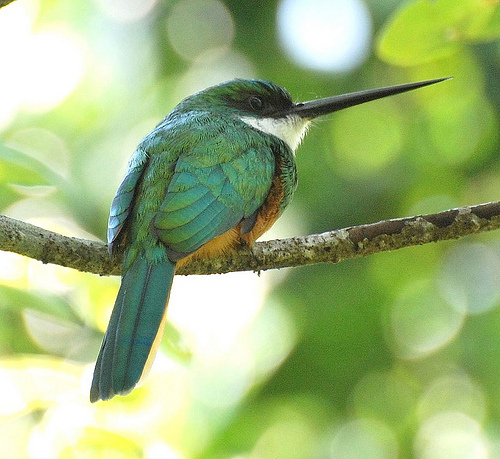
\includegraphics[trim={18mm 6mm 10mm 12mm},clip, width=\sizeP\textwidth]{opticam/images/eval/hihd/ILSVRC2012_val_00030507.JPEG}
    &
    \fig[\sizeS]{opticam/images/eval/hihd/ILSVRC2012_val_00030507JPEG_smap_opticam.png} 
    &                
    \fig[\sizeS]{opticam/images/eval/hihd/ILSVRC2012_val_00030507JPEG_smap_scorecam.png} \\
    staffordshire terrier&I$\uparrow$:62.1, D$\downarrow$:32.2&I$\uparrow$:93.4, D$\downarrow$:8.2&
    jacamar&I$\uparrow$:66.3, D$\downarrow$:17.3&I$\uparrow$:94.6, D$\downarrow$:9.9\\
    &AG$\uparrow$:41.3, AD$\downarrow$:0.0&AG$\uparrow$:0.0, AD$\downarrow$:0.3&
    &AG$\uparrow$:91.4, AD$\downarrow$:0.0&AG$\uparrow$:56.5, AD$\downarrow$:0.0\\
    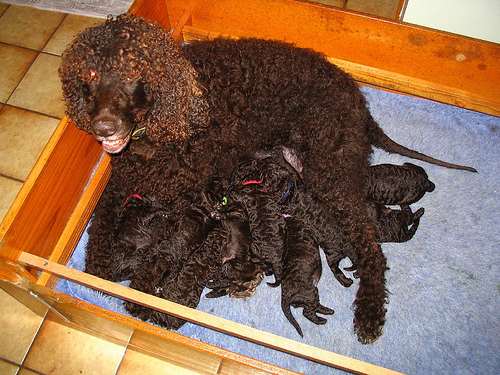
\includegraphics[trim={6mm 1mm 6mm 1mm},clip, width=\sizeP\textwidth]{opticam/images/eval/hihd/ILSVRC2012_val_00029237.JPEG}
    &
    \fig[\sizeS]{opticam/images/eval/hihd/ILSVRC2012_val_00029237JPEG_smap_opticam.png} 
    &     
    \fig[\sizeS]{opticam/images/eval/hihd/ILSVRC2012_val_00029237JPEG_smap_scorecam.png} &
    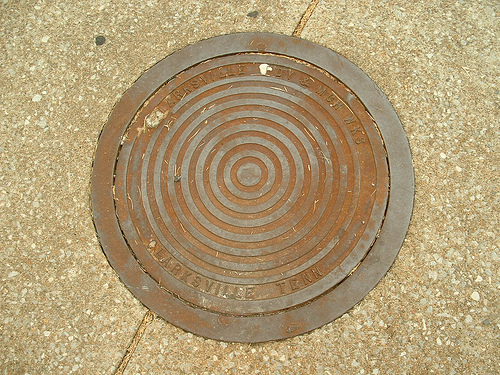
\includegraphics[trim={28mm 5mm 22mm 5mm},clip, width=\sizeP\textwidth]{opticam/images/eval/hihd/ILSVRC2012_val_00005077.JPEG}
    &
    \fig[\sizeS]{opticam/images/eval/hihd/ILSVRC2012_val_00005077JPEG_smap_opticam.png} 
    &          
    \fig[\sizeS]{opticam/images/eval/hihd/ILSVRC2012_val_00005077JPEG_smap_scorecam.png} \\
    Irish water spaniel&I$\uparrow$:52.6, D$\downarrow$:18.8&I$\uparrow$:90.5, D$\downarrow$:8.6&
    manhole cover&I$\uparrow$:65.8, D$\downarrow$:29.6&I$\uparrow$92.7, D$\downarrow$:9.1\\
    &AG$\uparrow$:86.4, AD$\downarrow$:0.0&AG$\uparrow$:65.1, AD$\downarrow$:0.0&
    &AG$\uparrow$:24.0, AD$\downarrow$:0.0&AG$\uparrow$:0.0, AD$\downarrow$:59.9\\
    % 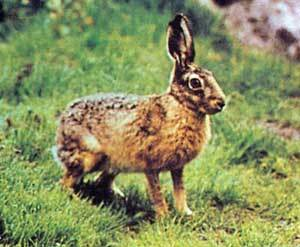
\includegraphics[trim={12mm 5mm 12mm 5mm},clip, width=\sizeP\textwidth]{ opticam/images/eval/hihd/ILSVRC2012_val_00003602.JPEG}
    % &              
    % \fig[\sizeS]{opticam/images/eval/hihd/ILSVRC2012_val_00003602JPEG_smap_opticam.png} 
    % & 
    % \fig[\sizeS]{opticam/images/eval/hihd/ILSVRC2012_val_00003602JPEG_smap_scorecam.png} \\
    % hare&I$\uparrow$:61.3, D$\downarrow$:21.2&I$\uparrow$91.3, D$\downarrow$:8.9\\
    % &AG$\uparrow$:93.7, AD$\downarrow$:0.0&AG$\uparrow$:0.0, AD$\downarrow$:0.6\\
    \end{tabular}
    \caption{\textbf{Failure examples} of Opti-CAM regarding insertion/deletion.}
    \label{fig:hihd}
    \end{figure}
    %------------------------------------------------------------------------------
% -------------------------------------------------------------------------------------------------
\noindent We argue that this is not a failure. As we will see in our localization experiment in 
\autoref{tab:localization} indicates, the background is useful in discriminating a class. Often, 
the network recognizes the background better than the object itself. For example, a gas pump is 
likely to be seen with a truck, and a hare is often seen on grass. Several parts of the object are 
highlighted by Opti-CAM for the worm fence, terrier dog, hare, and manhole cover. Finally, several 
instances of spaniel dog are found by Opti-CAM.\\